\documentclass[12pt]{article}
\textwidth 17cm \oddsidemargin 0cm \topmargin -2cm \textheight
24cm \footskip 1.5cm \usepackage{epsfig}
\usepackage{amsmath,graphicx,psfrag,pstcol,float,listings,color}
\usepackage{algorithm,algpseudocode,booktabs}
\usepackage{multirow}
\graphicspath{{./defn_files}}
\def\n{\noindent}
\def\u{\underline}
\def\hs{\hspace}
\newcommand{\thrfor}{.^{\displaystyle .} .}
\newcommand{\bvec}[1]{{\bf #1}}

\usepackage{listings}
\usepackage{pdfpages}
\usepackage{fancyvrb}

\definecolor{mGreen}{rgb}{0,0.6,0}
\definecolor{mGray}{rgb}{0.5,0.5,0.5}
\definecolor{mPurple}{rgb}{0.58,0,0.82}
\definecolor{backgroundColour}{rgb}{0.95,0.95,0.92}

\lstdefinestyle{Matlab}{
    backgroundcolor=\color{backgroundColour},   
    commentstyle=\color{mGreen},
    keywordstyle=\color{magenta},
    numberstyle=\tiny\color{mGray},
    stringstyle=\color{mPurple},
    basicstyle=\footnotesize,
    breakatwhitespace=false,         
    breaklines=true,                 
    captionpos=b,                    
    keepspaces=true,                 
    numbers=left,                    
    numbersep=5pt,                  
    showspaces=false,                
    showstringspaces=false,
    showtabs=false,                  
    tabsize=2,
    language=Matlab
}

\begin{document}

\vspace{0.3cm}
\rule{15.7cm}{0.5mm}


\begin{center}
{\hspace{0.6cm}\Large \textbf {Software First Interim Report}\\
}
\end{center}
\begin{table}[H]
\centering
\begin{tabular}{ p{1.5cm}p{5cm}p{6cm} p{6cm}} 
&Brian Sun & Trinity College & gs534 \\ 
&Charles Zhou & Magdalene College & yz493 \\ 
&Paul Zhao & Magdalene College & yz496 \\ 
\end{tabular}
\end{table}


\begin{center}
\rule{15.7cm}{0.5mm}
\end{center}

\section{Introduction}
\section{Teamwork Planning}
\section{EBNF}
\section{Possible Semantic Errors}
\section{Error Handling}
\section{Examples of Definition Files}

\section{Examples of Definition Files}
\subsection{Sequential Carry Adder}
\begin{figure}[h]
    \centering
    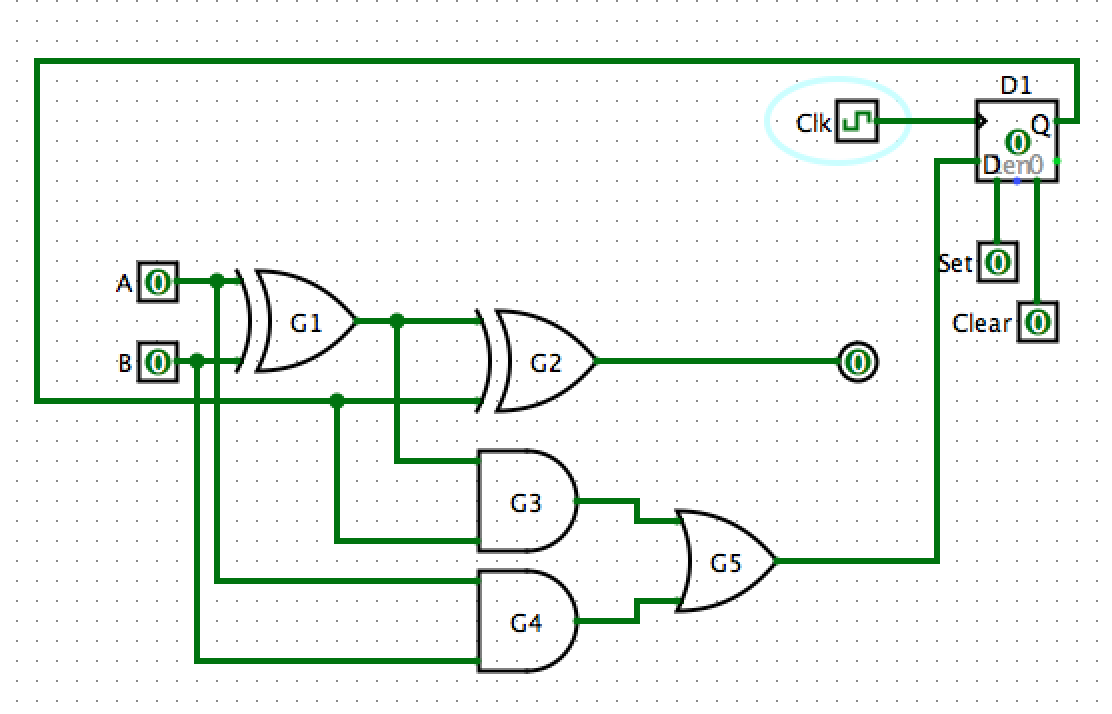
\includegraphics{sequential_carry_adder.png}
    \caption{circuit of a sequential carry adder}
\end{figure}

\VerbatimInput{sequential_carry_adder.txt}


\subsection{Binary Multiplier}
\begin{figure}[h]
    \centering
    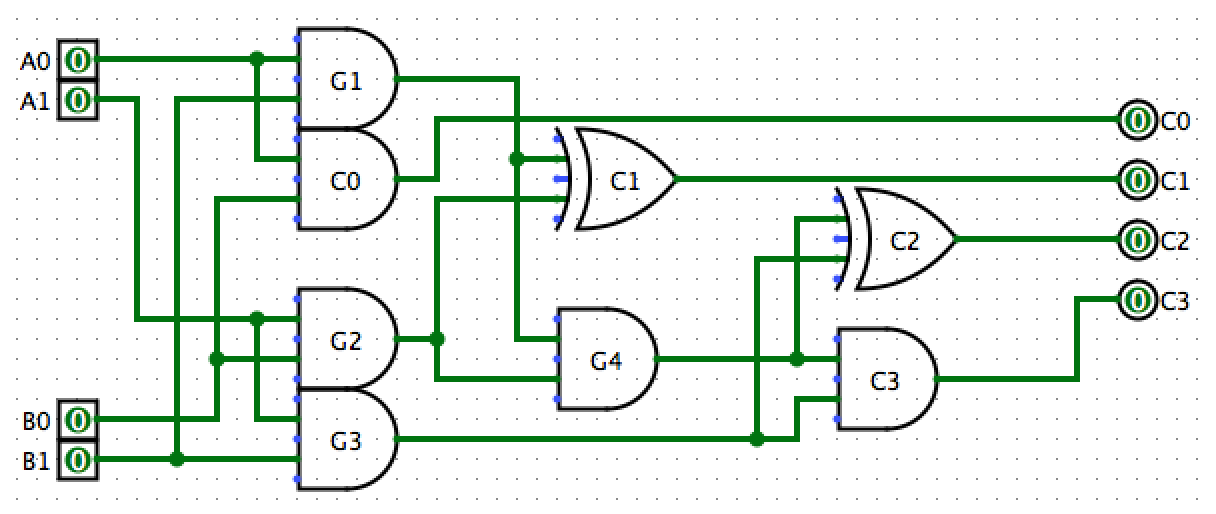
\includegraphics{bin_multiplier.png}
    \caption{circuit of a binary multiplier}
\end{figure}

\VerbatimInput{bin_multiplier.txt}




\end{document}



\end{document}